\documentclass[12pt,letterpaper,boxed,cm]{hmcpset}

\usepackage[margin=1in]{geometry}
\usepackage{mathtools}
\usepackage{mathrsfs}
\usepackage{graphicx}
\usepackage{cases}
\usepackage{enumitem}
\usepackage{soul}
\usepackage{listings}
\usepackage{changepage}

\name{John Gaskin}
\class{Computer Science 81}
\assignment{Homework 6}
\duedate{2/28/17}

\newcommand{\pn}[1]{\left( #1 \right)}
\newcommand{\abs}[1]{\left| #1 \right|}
\newcommand{\bk}[1]{\left[ #1 \right]}
\newcommand{\set}[1]{\left\{#1\right\}}
\newcommand{\ra}[0]{\rightarrow}
\newcommand{\cp}[0]{~\vdash~}
\newcommand{\turn}[0]{\,\vDash\,}
\newcommand{\EF}[0]{\text{EF}\,}
\newcommand{\AF}[0]{\text{AF}\,}
\newcommand{\EG}[0]{\text{EG}\,}
\newcommand{\AG}[0]{\text{AG}\,}

\begin{document}
\problemlist{1, 2, 3, 4, 5, 6, 7}
\textbf{Models}\\
You have seen models for propositional logic (an assignment of true/false values to propositional variables) and modes for predicate logic (which further specify sets of individuals and define the meaning of relations and functions).\\\\
Let us say a model $M$ for CTL formulas consists of
\begin{itemize}
    \item a set of states $S$ (representing possible ``states'' or ``configurations'' of a system)
    \item a binary relation ``$\ra$'' between states (a specification of whether $s \ra s'$ is true or false, for any two states $s\in S$ and $s'\in S$, meaning the system can go from state $s$ directly to state $s'$)
    \item a specification of what predicate-logic formulas are true in \ul{each} state $s$
\end{itemize}
Normally we assume that for every state $s$, there is at least one \emph{next} state $s'$ such that $s \ra s'$. If our system is not totally deterministic, $s$ might have \emph{many} such next states (e.g., $s \ra s'$ and $s\ra s''$ are both true, even when $s'$ and $s''$ are different states)\\\\
We write $s_1 \ra s_2 \ra s_3$  to mean $(s_1 \ra s_2) \land (s_2 \ra s_3)$, and so on.\\\\
Given a model $M$ and a state $s_1$, we write $M,s_1 \turn \phi$  to mean that formula $\phi$ is true in state $s$.\\
This relation is defined as follows:
\begin{center}
    \begin{tabular}{l l}
        $M, s_1 \turn \top$           & always \\
        $M,s_1 \turn \phi$            & if $\phi$ is a predicate-logic formula (no EF,AG,etc.)
                                       and $M$ says that $\phi$ is true in state $s_1$ \\
        $M,s_1 \turn \neg\phi$        & if $(M,s_1 \turn \phi)$ does not hold. \\
        $M,s_1 \turn \phi \land \psi$ & if $M,s_1 \turn \phi$ and $M,s_1 \turn \psi$ \\
        $M,s_1 \turn \phi \lor \psi$  & if $ M,s_1 \turn \phi$ or $ M,s_1 \turn \psi$ \\
        $M,s_1 \turn \phi \ra \psi$   & if $(M,s_1 \turn \phi)$ does not hold or $(M,s_1 \turn \psi)$ does \\
        $M,s_1 \turn \EF \phi$        & if there \ul{exists} a path $s_1 \ra s_2 \ra s_3 \ra \cdots$  such that
                                       $M,s_j \turn \phi$  holds for \ul{some} $j \ge 1$. \\
        $M,s_1 \turn \AF \phi$        & if for \ul{every} path $s_1 \ra s_2 \ra s_3 \ra \cdots M,s_j \turn \phi$ 
                                       holds for \ul{some} $j \ge 1$. \\
        $M,s_1 \turn \EG \phi$        & if there \ul{exists} a path $s_1 \ra s_2 \ra s_3 \ra \cdots$  such that
                                       $M,s_j \turn \phi$  holds for \ul{every} $j \ge 1$. \\
        $M,s_1 \turn \AG \phi$        & if for \ul{every} path $s_1 \ra s_2 \ra s_3 \ra \cdots$,  $M,s_j \turn \phi$  
                                       holds for \ul{every} $j \ge 1$.
    \end{tabular}
\end{center}

\textbf{Note:}  ``the future includes the present'' in the last four definitions.\\
For example, $M,s_1 \turn \EF p$  is true if $p$ is true in state $s_1$ itself, 
even if it's never again true in the future (i.e., if $\neg p$ holds for all states reachable from $s_1$).
\newpage

\begin{problem}[1.]
    [15 points] Using the above definitions, which of the following CTL formulas are equivalent (both true or both false) for every model $M$ and every state $s$?  Carefully justify your answers (using complete sentences).
    \begin{enumerate}[label=\Alph*.]
        \item $(\EF \phi) \lor (\EF \psi)$   and    $\EF (\phi \lor \psi)$
        \item $(\AF \phi) \lor (\AF \psi)$    and   $\AF (\phi \lor \psi)$
        \item $\EF (\neg\phi)$   and    $\neg(\AF \phi)$.
    \end{enumerate}
\end{problem}

\begin{solution}
    \vfill
\end{solution}
\newpage

\begin{problem}[2.]
    [24 points] Consider the following piece of C/C++/Java-style code:
    \begin{lstlisting}[mathescape]
int a[100] = $\set{ 0, 0, 0, \ldots, 0 }$;  // Array is initially 100 zeros

// loop forever
while (true) {
    int k = get_input(); // Assume the user always enters a number
                         //      between 0 and 99 inclusive!

    if (a[k] == 1) {
         // Reset the array back to all zeros
         for (int i = 0; i < 100; ++i)
              a[i] = 0;
    } else {
         // Set the k-th element of the array to 1
         a[k] = 1;
    }
}
    \end{lstlisting}
    We can view this program as describing a CTL model where the states are the possible memory contents of the program, the $\ra$ relation describes how memory changes from moment to moment over time in this program, and our predicate-logic formulas are claims about the contents of memory in a particular program state.\\\\
    Which of the following logical propositions are true (starting at the beginning of the program)?  Explain your answers; you do not need to provide a full formal proof, but your explanation should be clear and convincing.
    \begin{enumerate}[label=\Alph*.]
        \item $\AG  (a[42] == 0)$
        \item $\displaystyle \AG\pn{\sum_{j=0}^{j<100}a\bk{j}<100}$~~~~~[careful]
        \item $\EF  (a[42] == 1)$
        \item $\AF  (a[42] == 1)$
        \item $\EG  (a[42] == 0)$
        \item $\AG  (\AF  (a[42] == 0))$
        \item $\AG  (\EF  (a[42] == 1))$
        \item $\EF  (AG  (a[42] == 0))$
    \end{enumerate}
\end{problem}

\begin{solution}
    \vfill
\end{solution}
\newpage
\hrule
~\\
Logician Raymond Smullyan passed away this past February 6, at the age of 97. After his very promising career as a pianist was cut short by tendonitis, he switched back to mathematics. There he did very influential work in the study of logic and formal systems: he is credited with improving and popularizing the use of Tableau-style proofs, and with extending and generalizing G\"odel's Incompleteness Theorem.\\\\
He was also the author of many wonderful books of puzzles focused on logic and computability, including \emph{What is the Name of this Book?, To Mock a Mockingbird}, and \emph{The Lady or the Tiger}. In his memory, here is a small sampling of his puzzles. (Make it very clear what your answer is, and include a justification.)
\hrule
\begin{problem}[3.]
    [4 points] ``In Shakespeare's \emph{Merchant of Venice} Portia had three caskets–gold, silver, and lead–inside one of which was Portia's portrait. The suitor was to choose one of the caskets, and if he was lucky enough (or wise enough) to choose the one with the portrait, then he could claim Portia as his bride. On the lid of each casket was an inscription to help the suitor choose wisely.''
    \begin{enumerate}[label=\Alph*.]
        \item Now, suppose Portia wished to choose her husband not on the basis of virtue, but simply on the basis of intelligence. She had the following inscriptions put on the caskets.
        \begin{center}
            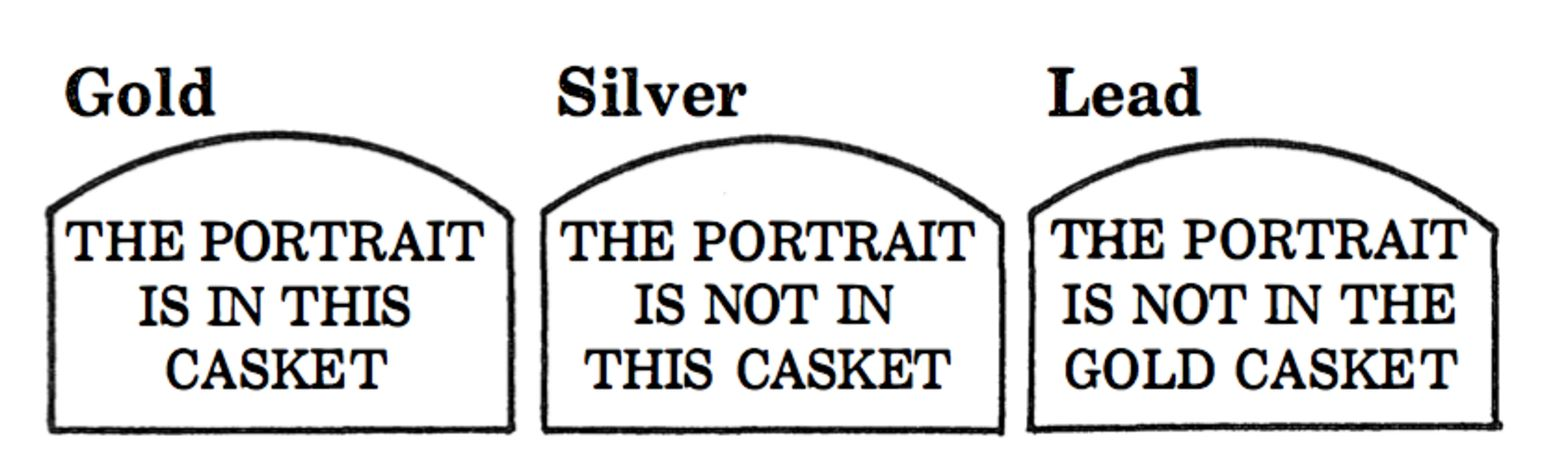
\includegraphics[scale=0.25]{01.JPG}
        \end{center}
        Portia explained to the suitor that of the three statements, at most one was true.  Which casket should the suitor choose?
        \item Portia's suitor chose correctly, so they married and lived quite happily–at least for a while. Then, one day, Portia had the following thoughts: ``Though my husband showed some intelligence in choosing the right casket, the problem wasn't really that difficult. Surely, I could have made the problem harder and gotten a really clever husband.'' So she forthwith divorced her husband and decided to get a clev­erer one.  This time she had the following inscriptions put on the caskets:
        \begin{center}
            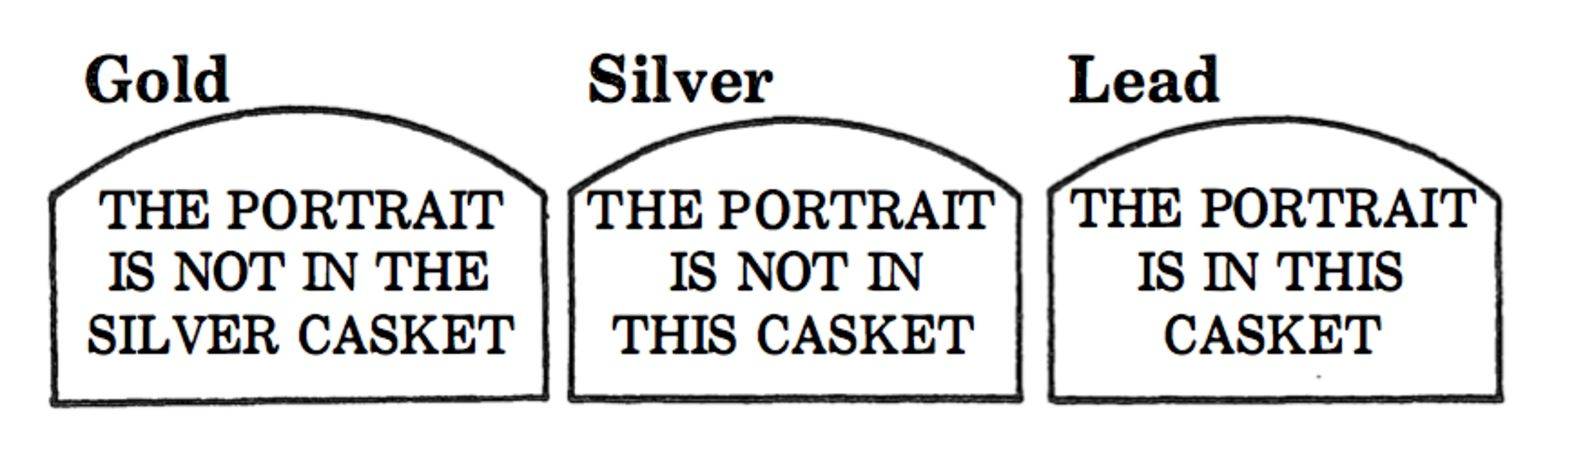
\includegraphics[scale=0.25]{02.JPG}
        \end{center}
        Portia explained to the suitor that at least one of the three statements was true and that at least one of them was false.  Which casket contains the portrait?
    \end{enumerate}
\end{problem}

\begin{solution}
    \vfill
\end{solution}
\newpage

\begin{problem}[4.]
    [8 points] [On the Island of Knights and Knaves, every inhabitant is either a \emph{knight} or a \emph{knave}; knights make \ul{only} true statements and knaves \ul{only} false ones.] ``Inspector Craig of Scotland Yard was called to the Island of Knights and Knaves to help find a criminal named Arthur York. What made the process difficult was that it wasn't known if Arthur York was a knight or a knave.''
    \begin{enumerate}[label=\Alph*.]
        \item One suspect was arrested. Here is a transcript of the trial; is the defendant Arthur York?
        \begin{adjustwidth}{1cm}{}
            Craig: What do you know about Arthur York?\\
            Defendant: Arthur York once claimed that I was a knave.\\
            Craig: Are you by any chance Arthur York?\\
            Defendant: Yes.
        \end{adjustwidth}
        \item Another suspect was arrested and brought to trial. Here is a transcript; is he Arthur York?
        \begin{adjustwidth}{1cm}{}
            Craig: The last suspect claimed to be Arthur York! Did you ever claim to be Arthur York?\\
            Defendant: No.\\
            Craig: Did you ever claim that you are not Arthur York?\\
            Defendant: Yes.
        \end{adjustwidth}
        \item A third suspect was arrested and brought to trial. He brought with him his local defense attorney, and the two made the following statements in court. Is it Arthur York?
        \begin{adjustwidth}{1cm}{}
            Defense Attorney:  My client is indeed a knave, but he is not Arthur York.\\
            Defendant: My attorney always tells the truth!
        \end{adjustwidth}
        \item Craig met a native who said, “This is not the first time I have said what I am now saying.” Was the native a knight or a knave?
    \end{enumerate}
\end{problem}

\begin{solution}
    \vfill
\end{solution}
\newpage

\begin{problem}[5.]
    [8 points] ``At the time I was in Transylvania, about half the inhabitants were human and half were vampires. The humans and vampires are indistinguishable in their out­ward appearance, but the humans (at least in Transylvania) always tell the truth and the vampires always lie. What enormously complicates the situation is that half the in­habitants of Transylvania are totally insane and completely deluded in their beliefs–all true propositions they believe to be false and all false propositions they believe to be true. The other half are completely sane and know which pro­positions are true and which ones false. Thus the inhabi­tants of Transylvania are of four types: (1) sane humans; (2) insane humans; (3) sane vampires; (4) insane vampires. Whatever a sane human says is true; whatever an insane human says is false; whatever a sane vampire says is false; and whatever an insane vampire says is true. For example, a sane human will say that two plus two equals four; an insane human will say it doesn't (because he really believes it doesn't); a sane vampire will also say it doesn't (because he knows it does and then lies); an insane vampire will say it does (he believes it doesn't, and then lies about what he believes).''
    \begin{enumerate}[label=\Alph*.]
        \item I once met a Transylvanian who said, “I am human or I am sane."  What type was he?
        \item Another inhabitant said, ``I am not a sane human.'' What type was he?
        \item I once met an inhabitant and asked him, ``Are you an insane vampire?'' He answered ``Yes'' or ``No,'' and I knew what he was. What was he?
        \item Suppose a Transylvanian said, ``"If I am either a sane human or an insane vampire, then Count Dracula is still alive.'' Could it then be determined whether Dracula is still alive?

    \end{enumerate}
\end{problem}

\begin{solution}
    \vfill
\end{solution}
\newpage

\begin{problem}[6.]
    [8 points] ``Inspector Craig dreamed that he spent nine days in a region in which dwelled gods, demons, and mortals. The gods, of course, always told the truth, and the demons always lied. As to the mortals, half were knights and half were knaves; knights always tell the truth, and knaves always lie.''
    \begin{enumerate}[label=\Alph*.]
        \item Craig dreamed that on the first day he met a dweller of the region who looked as if he might be a god, though Craig could not be sure. The dweller evidently guessed Craig's thoughts, smiled, and made a statement to reassure him. From this statement, Craig \emph{knew} he was in the presence of a god. Can you supply such a statement?
        \item On the second day, Craig met a terrifying-looking being who had every appearance of being a demon.``What sort of being are you?'' asked Craig, in some alarm. The being answered, and Craig then realized that he was confronting not a demon, but a knave. What could the being have answered?
        \item On the fourth day, Craig met a being who made the following two statements:
        \begin{itemize}
            \item A god once claimed that I am a demon.
            \item No knight has ever claimed that I am a knave.
        \end{itemize}
        What sort of being was he?
        \item On the eight day, Craig met a being who had every appearance of being the god Thor. The being made a statement, and Craig then knew it must \emph{be} Thor. What statement could Thor have made?
    \end{enumerate}
\end{problem}

\begin{solution}
    \vfill
\end{solution}
\newpage

\begin{problem}[7.]
    [1 easy point] Answer this quick survey when you’re done:
    \begin{enumerate}[label=\Alph*.]
        \item How long (in hours) did you spend working on this assignment?
        \item What was the most interesting thing you learned while answering these problems? (We're sure there was \emph{something} you learned.)
    \end{enumerate}
    
\end{problem}

\begin{solution}
    \vfill
\end{solution}

\end{document}
